% Author: Izaak Neutelings (November 2020)
\documentclass[border=3pt,tikz]{standalone}
\usepackage{siunitx}
\usepackage{physics}
\usepackage{tikz}
\usepackage[outline]{contour} % glow around text
\usetikzlibrary{patterns,decorations.pathmorphing}
\usetikzlibrary{arrows.meta}
\tikzset{>=latex}
\contourlength{1.1pt}

\colorlet{mydarkblue}{blue!50!black}
\colorlet{myblue}{blue!30}
\colorlet{myred}{red!65!black}
\colorlet{vcol}{green!45!black}
\colorlet{watercol}{blue!80!cyan!10!white}
\colorlet{darkwatercol}{blue!80!cyan!20!white}
\colorlet{metalcol}{blue!40!black!10!white}
\tikzstyle{force}=[->,myred,very thick,line cap=round]
\tikzstyle{vvec}=[->,very thick,vcol,line cap=round]
\tikzstyle{ground}=[preaction={fill,top color=black!10,bottom color=black!5,shading angle=20},
                    fill,pattern=north east lines,draw=none,minimum width=0.3,minimum height=0.6]
\tikzstyle{mass}=[line width=0.6,red!30!black,fill=red!40!black!10,rounded corners=1,
                  top color=red!40!black!20,bottom color=red!40!black!10,shading angle=20]
\tikzstyle{rope}=[brown!70!black,line width=1.2,line cap=round] %very thick
\tikzstyle{piston}=[blue!50!black,top color=blue!30,bottom color=blue!50,middle color=blue!20,shading angle=0]
\tikzstyle{water}=[draw=mydarkblue,top color=watercol!90,bottom color=watercol!90!black,shading angle=5]
\tikzstyle{vertical water}=[water,
  top color=watercol!90!black!90,bottom color=watercol!90!black!90,middle color=watercol!80,shading angle=90]
\tikzstyle{dark water}=[draw=mydarkblue,top color=darkwatercol,bottom color=darkwatercol!80!black,shading angle=5]
\tikzstyle{metal}=[draw=metalcol!20!black,top color=metalcol,bottom color=metalcol!90!black,shading angle=10]
\tikzstyle{width}=[{Latex[length=3,width=3]}-{Latex[length=3,width=3]}]
\tikzstyle{force}=[->,myred,thick,line cap=round]
\tikzstyle{Fproj}=[force,myred!40]
\newcommand{\vbF}{\vb{F}}
\tikzstyle{rope}=[brown!20!black,double=brown!70!black,double distance=1,line width=0.3] %very thick
%\def\rope#1{ \draw[black,line width=2.3] #1; \draw[rope] #1; }
\def\tick#1#2{\draw[thick] (#1)++(#2:0.1) --++ (#2-180:0.2)}



\begin{document}


% BUOYANT FORCE
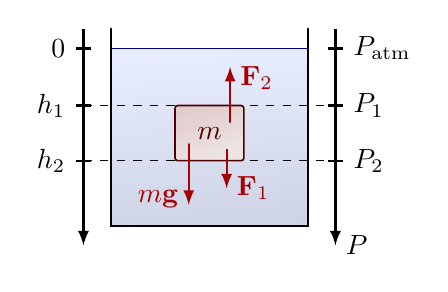
\begin{tikzpicture}
  \def\H{2.5}      % container height
  \def\W{2.5}      % container width
  \def\h{0.9*\H}   % water level height
  \def\my{0.33*\H} % mass y position
  \def\mh{0.28*\H} % mass height
  \def\mw{0.35*\H} % mass width
  
  % CONTAINER
  \draw[water] (-\W/2,0) rectangle++ (\W,\h); %,rounded corners=2
  \draw[thick,line cap=round] (-\W/2,\H) |-++ (\W,-\H) --++ (0,\H);
  
  % MASS
  \draw[dashed]
    (-0.64*\W,\my) -- (0.64*\W,\my)
    (-0.64*\W,\my+\mh) -- (0.64*\W,\my+\mh);
  \draw[mass] (-\mw/2,\my) rectangle++ (\mw,\mh) node[midway] {$m$};
  \draw[force] (0.30*\mw,\my+0.7*\mh) --++ (0,\mh) node[below=4,right=0] {$\vbF_2$};
  \draw[force] (0.25*\mw,\my+0.2*\mh) --++ (0,-0.7*\mh) node[right=0] {$\vbF_1$};
  \draw[force] (-0.3*\mw,\my+0.3*\mh) --++ (0,-1.1*\mh) node[above=2,left=0] {$m\vb{g}$};
  
  % AXIS depth
  \draw[->,thick]
    (-0.64*\W,\H) --++ (0,-1.1*\H);
  \tick{-0.64*\W,\h}{0} node[left] {$0$};
  \tick{-0.64*\W,\my+\mh}{0} node[left] {$h_1$};
  \tick{-0.64*\W,\my}{0} node[left] {$h_2$};
  
  % AXIS pressure
  \draw[->,thick]
    (0.64*\W,\H) --++ (0,-1.1*\H) node[right] {$P$};
  \tick{0.64*\W,\h}{180} node[right] {$P_\mathrm{atm}$};
  \tick{0.64*\W,\my+\mh}{180} node[right] {$P_1$};
  \tick{0.64*\W,\my}{180} node[right] {$P_2$};
  
\end{tikzpicture}


% BUOYANT FORCE
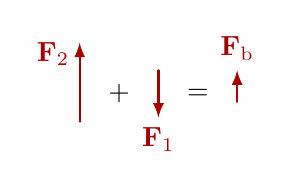
\begin{tikzpicture}
  \def\H{2.0}      % container height
  \def\W{1.0}      % total width
  \def\h{0.9*\H}   % water level height
  \def\mh{0.28*\H} % mass height
  \def\mw{0.35*\H} % mass width
  \def\F{1.0}      % force
  
  % MASS
  \draw[force] (-\W,-0.35*\F) --++ (0,\F) node[below=4,left=0] {$\vbF_2$};
  \node at (-\W/2,0) {$+$};
  \draw[force] (0,0.3*\F) --++ (0,-0.6*\F) node[below=0] {$\vbF_1$};
  \node at (\W/2,0) {$=$};
  \draw[force] (\W,-0.1*\F) --++ (0,0.4*\F) node[above=0] {$\vbF_\mathrm{b}$};
  %\draw[mass] (0,0) circle(0.05*\F) node[left=1] {$m$} (\W,0) circle(0.05*\F);
  
\end{tikzpicture}


% BUOYANT FORCE - floating
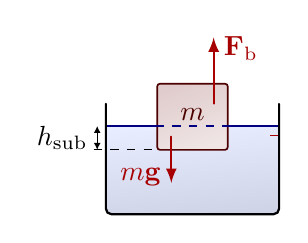
\begin{tikzpicture}
  \def\H{1.4}          % container height
  \def\W{2.2}          % container width
  \def\h{0.8*\H}       % water level height
  \def\my{\h-0.36*\mh} % mass y position
  \def\mh{0.60*\H}     % mass height
  \def\mw{0.64*\H}     % mass width
  \def\F{0.60*\H}      % force magnitude
  
  % CONTAINER
  \draw[water,rounded corners=2] (-\W/2,\h) |-++ (\W,-\h) --++ (0,\h);
  \draw[mydarkblue] (-\W/2,\h) --++ (\W,0);
  \draw[myred] (\W/2,{\h-(\h-(\my))*\mw/\W}) --++ (-0.05*\W,0);
  
  % MASS
  \draw[dashed] (-0.57*\W,\my) --++ (0.5*\W,0);
  \draw[{Latex[length=2.5,width=2.5]}-{Latex[length=2.5,width=2.5]}]
    (-0.55*\W,\h) --++ (0,{\my-\h}) node[midway,left=0] {$h_\mathrm{sub}$};
  \draw[mass] (-\mw/2,\my) rectangle++ (\mw,\mh) node[midway,above=-5] {$m$};
  \draw[force] (0.30*\mw,\my+0.7*\mh) --++ (0,\F) node[below=4,right=0] {$\vbF_\mathrm{b}$};
  \draw[force] (-0.3*\mw,\my+0.2*\mh) --++ (0,-0.7*\F) node[above=2,left=0] {$m\vb{g}$};
  \draw[mydarkblue,dashed] (-\W/2,\h) --++ (\W,0);
  \draw[thick,rounded corners=2,line cap=round] (-\W/2,\H) |-++ (\W,-\H) --++ (0,\H);
  
\end{tikzpicture}


% BUOYANT FORCE - floating
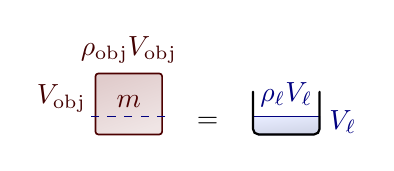
\begin{tikzpicture}
  \def\H{1.8}        % container height
  \def\W{2.0}        % container width
  \def\h{0.8*\H}     % water level height
  \def\my{-0.20*\mh} % mass y position
  \def\mh{0.43*\H}   % mass height
  \def\mw{0.47*\H}   % mass width
  \draw[mass] (-\mw/2,-\mh/2) rectangle++ (\mw,\mh) node[midway,above=-5] {$m$};
  \draw[mydarkblue,dashed] (0.55*\mw,\my) --++ (-1.2*\mw,0);
  \node[above=2,left,myred!40!black] at (-\mw/2,0) {$V_\mathrm{obj}$};
  \node at (\W/2,-0.3*\mh) {$=$};
  \draw[water,rounded corners=2] (\W-\mw/2,\my) |-++ (\mw,-\mh/2-\my) --++ (0,\mh/2+\my);
  \draw[mydarkblue] (\W-\mw/2,\my) --++ (\mw,0) node[below=2,right] {$V_\ell$};
  \draw[thick,rounded corners=2,line cap=round]
    (\W-\mw/2,0.2*\mh) |-++ (\mw,-0.7*\mh) --++ (0,0.7*\mh);
  \node[above=0,mydarkblue] at (\W,\my) {$\rho_\ell V_\ell$};
  \node[above=0,myred!40!black] at (0,\mh/2) {$\rho_\mathrm{obj} V_\mathrm{obj}$};
\end{tikzpicture}


% BUOYANT FORCE - weights
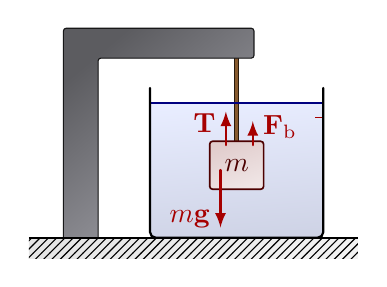
\begin{tikzpicture}
  \def\H{1.9}         % container height
  \def\W{2.2}         % container width
  \def\h{0.9*\H}      % water level height
  \def\my{\h-1.8*\mh} % mass y position
  \def\mh{0.32*\H}    % mass height
  \def\mw{0.36*\H}    % mass width
  
  % GROUND
  \draw[water,rounded corners=2] (-\W/2,\h) |-++ (\W,-\h) --++ (0,\h);
  \draw[ground] (-1.2*\W,0) rectangle++ (1.9*\W,-0.14*\H);
  \draw[rope] (0,1.3*\H) -- (0,\my+0.9*\mh);
  \fill[draw=metalcol!10!black,top color=metalcol!40!black,bottom color=metalcol!70!black,shading angle=40,rounded corners=1]
    (-1.0*\W,0) |- (0.1*\W,1.4*\H) |- (-0.8*\W,1.2*\H) |- (-0.8*\W,0);
  
  % CONTAINER
  \draw[thick] (-1.2*\W,0) --++ (1.9*\W,0);
  \draw[mydarkblue] (-\W/2,\h) --++ (\W,0);
  \draw[myred] (\W/2,{\h-\mh*\mw/\W}) --++ (-0.05*\W,0);
  
  % MASS
  \draw[mass] (-\mw/2,\my) rectangle++ (\mw,\mh) node[midway] {$m$};
  \draw[force] (0.30*\mw,\my+0.92*\mh) --++ (0,0.5*\mh) node[below=2,right=0] {$\vbF_\mathrm{b}$};
  \draw[force] (-0.2*\mw,\my+0.92*\mh) --++ (0,0.7*\mh) node[below=4,left=0] {$\vb{T}$};
  \draw[force] (-0.3*\mw,\my+0.40*\mh) --++ (0,-1.2*\mh) node[above=3,left=0] {$m\vb{g}$};
  \draw[thick,rounded corners=2,line cap=round] (-\W/2,\H) |-++ (\W,-\H) --++ (0,\H);
  
\end{tikzpicture}



% BUOYANCY plot
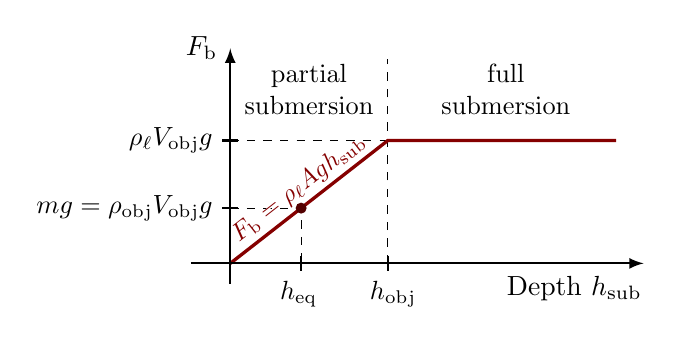
\begin{tikzpicture}
  \def\xmax{5.0}
  \def\ymax{2.6}
  \def\xc{0.40*\xmax} % fully submerged
  \def\yc{0.60*\ymax} % fully submerged
  \def\xe{0.18*\xmax} % equilibrium
  \def\ye{\yc*\xe/(\xc)}    % equilibrium
  \draw[dashed] (\xc,0) --++ (0,\ymax);
  \draw[dashed] (0,\yc) --++ (\xc,0);
  \draw[dashed] (0,{\ye}) -| (\xe,0);
  \draw[myred!80!black,very thick]
    (0,0) -- (\xc,\yc)
    node[scale=0.9,midway,right=1,above=-1,rotate={atan2(\yc,\xc)}] {\contour{white}{$F_\mathrm{b} = \rho_\ell Agh_\mathrm{sub}$}}
    -- (0.98*\xmax,\yc);
    %node[scale=0.9,midway,above=-2] {$F_\mathrm{b} = ...$};
  \fill[myred!50!black] (\xe,{\ye}) circle(0.07);
  \draw[->,thick] (-0.1*\xmax,0) -- (1.05*\xmax,0) node[right=4,below left=1] {Depth $h_\mathrm{sub}$};
  \draw[->,thick] (0,-0.1*\ymax) -- (0,1.05*\ymax) node[left=1] {$F_\mathrm{b}$};
  %\draw[->,thick] (0,-0.1*\ymax) -- (0,\ymax) node[above left=1,rotate=90] {Buoyant force $F_\mathrm{b}$};
  \tick{0,\yc}{0} node[scale=0.95,left=0] {$\rho_\ell V_\mathrm{obj}g$};
  \tick{0,{\ye}}{0} node[scale=0.95,left=0] {$mg=\rho_\mathrm{obj} V_\mathrm{obj}g$};
  \tick{\xc,0}{90} node[scale=0.95,right=2,below] {$h_\mathrm{obj}$};
  \tick{\xe,0}{90} node[scale=0.95,left=1,below] {$h_\mathrm{eq}$};
  \node[align=center,scale=0.95] at (\xc/2,0.85*\ymax) {partial\\submersion};
  \node[align=center,scale=0.95] at ({(\xmax+\xc)/2},0.85*\ymax) {full\\submersion};
\end{tikzpicture}



\end{document}
